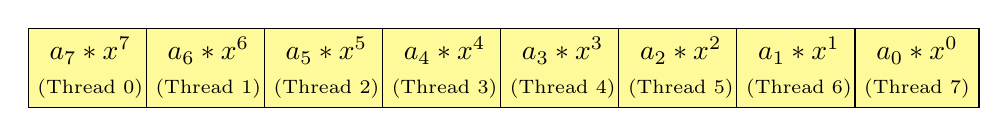
\begin{tikzpicture}[level/.style={sibling distance=60mm/#1}]

\def\HEIGHT{1}
\def\WIDTH{1.5}

% leaves
\node (rect) at (0*\WIDTH,0) [draw,minimum width=\WIDTH cm,minimum height=\HEIGHT cm, fill=yellow!40, align=center] (a0) {$a_7*x^7$\\\scriptsize{(Thread 0)}};
\node (rect) at (1*\WIDTH,0) [draw,minimum width=\WIDTH cm,minimum height=\HEIGHT cm, fill=yellow!40, align=center] (a1) {$a_6*x^6$\\\scriptsize{(Thread 1)}};
\node (rect) at (2*\WIDTH,0) [draw,minimum width=\WIDTH cm,minimum height=\HEIGHT cm, fill=yellow!40, align=center] (a2) {$a_5*x^5$\\\scriptsize{(Thread 2)}};
\node (rect) at (3*\WIDTH,0) [draw,minimum width=\WIDTH cm,minimum height=\HEIGHT cm, fill=yellow!40, align=center] (a3) {$a_4*x^4$\\\scriptsize{(Thread 3)}};
\node (rect) at (4*\WIDTH,0) [draw,minimum width=\WIDTH cm,minimum height=\HEIGHT cm, fill=yellow!40, align=center] (a4) {$a_3*x^3$\\\scriptsize{(Thread 4)}};
\node (rect) at (5*\WIDTH,0) [draw,minimum width=\WIDTH cm,minimum height=\HEIGHT cm, fill=yellow!40, align=center] (a5) {$a_2*x^2$\\\scriptsize{(Thread 5)}};
\node (rect) at (6*\WIDTH,0) [draw,minimum width=\WIDTH cm,minimum height=\HEIGHT cm, fill=yellow!40, align=center] (a6) {$a_1*x^1$\\\scriptsize{(Thread 6)}};
\node (rect) at (7*\WIDTH,0) [draw,minimum width=\WIDTH cm,minimum height=\HEIGHT cm, fill=yellow!40, align=center] (a7) {$a_0*x^0$\\\scriptsize{(Thread 7)}};

\end{tikzpicture}